\documentclass[a4paper,10pt]{article}

\title{Rapport de robotique mobile Hovercraft}

\author{TERRIE Corentin - BELLOC Thomas \\ CROS Bastien - ABLAJ Yassine \\ SZAFIR Michael - BOUKHALFA Yannis \\ MONNIER Matthias}

\date{\today}

\usepackage[utf8]{inputenc}
\usepackage[french]{babel} 
\usepackage{lmodern} % Pour changer le pack de police
\usepackage{makeidx}
\usepackage{fancyhdr}
\usepackage{graphicx}
\usepackage[lofdepth,lotdepth]{subfig}
\usepackage{float}
\usepackage{hyperref}
%---------------------------------------------------------
\usepackage{listings}
\usepackage{textcomp}
\usepackage{bigcenter}
% JAVA en couleur ;-)- -----------------------------------
%\lstset{
%language=Java,
%basicstyle=\normalsize, % ou ça==> basicstyle=\scriptsize,
%upquote=true,
%aboveskip={1.5\baselineskip},
%columns=fullflexible,
%showstringspaces=false,
%extendedchars=true,
%breaklines=true,
%showtabs=false,
%showspaces=false,
%showstringspaces=false,
%identifierstyle=\ttfamily,
%keywordstyle=\color[rgb]{0,0,1},
%commentstyle=\color[rgb]{0.133,0.545,0.133},
%stringstyle=\color[rgb]{0.627,0.126,0.941},
%}


%----------------------------------------------------------

\begin{document}

\makeatletter
  \begin{titlepage}
  \centering
      {\Large \textsc{École Universitaire Polytechnique de Montpellier}}\\
      \textsc{Microélectronique et Automatique - Électronique et Informatique Industrielle }\\
    \noindent\hrulefill 
    \\
    \vspace{1.5cm}
      {\large	\@date\\}
    \vspace{1.5cm}
       {\huge \textbf{\@title}} \\
	
	\vspace{0.7cm}
      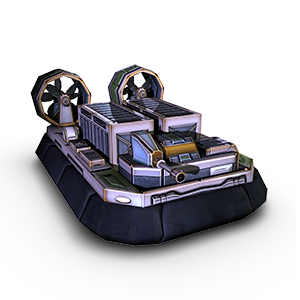
\includegraphics[scale=0.38]{head.png}\\

    \vspace{2em}
        {\large \@author} \\
    
    \vspace{2.6cm}
        
\includegraphics[height=0.15\textheight]{mea.jpg}
        \hfill
        
\includegraphics[height=0.15\textheight]{um.png}
  \end{titlepage}
\makeatother
\tableofcontents
\clearpage


%-------------------------------------------------------------------------------

\section{Introduction}



\subsection{Répartition des tâches}




%-------------------------------------------------------------------------------------------------------------

\section{Étude de fonctionnement général d'un aéroglisseur}


%-------------------------------------------------------------------------------------------------------------

\section{Simulateur}
\subsection{Modèle}
\subsection{Implémentation}
\subsubsection{Schéma de commande}
Le schéma global utilisé pour le simulateur est le suivant :

\begin{figure}[H]
\bigcenter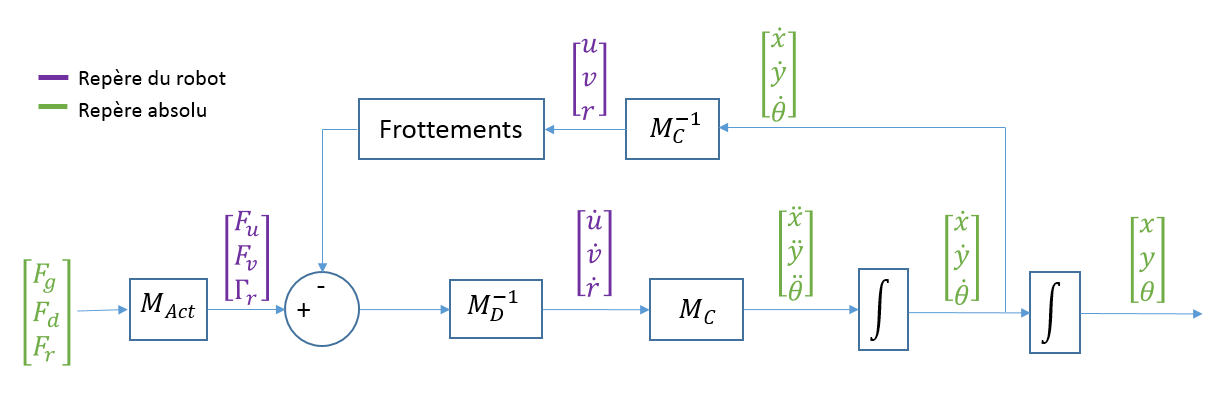
\includegraphics[scale=0.5]{images/commande.png}
\caption{Schéma général de notre simulateur.}
\end{figure}

On commande notre système en choisissant la force appliquée par chaque moteur. Fr est la force de sustentation. $F_g$ et $F_d$ sont les moteurs droit et gauche. On obtient en sortie de notre simulateur la position et l’orientation de notre aéroglisseur dans le plan $(x,y)$. 

\subsubsection{Matrice d'actionnement}
\begin{figure}[H]
\bigcenter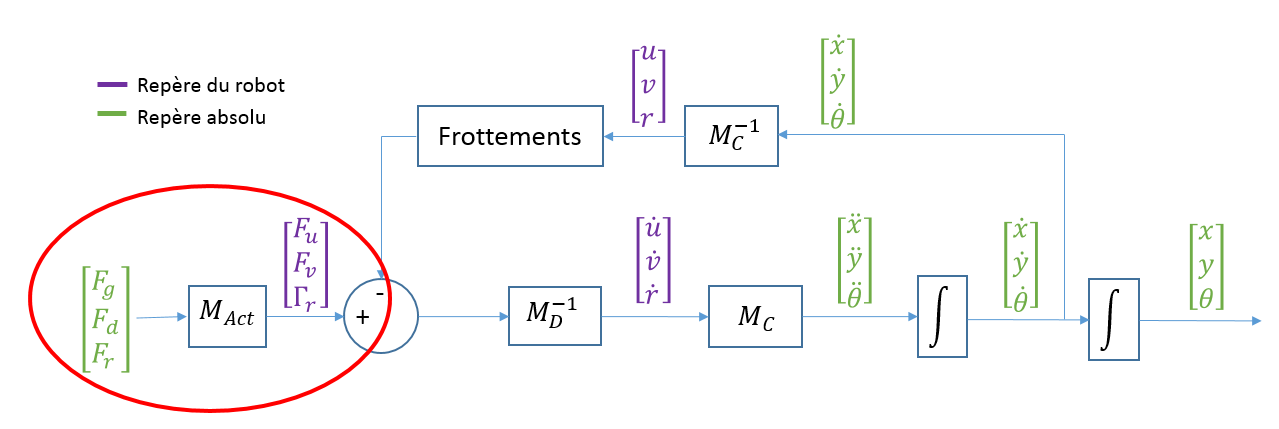
\includegraphics[scale=0.5]{images/matrice_actionnement.png}
\caption{Matrice d'actionnement.}
\end{figure}

Pour passer des forces dans le repère absolu à celles dans le repère du robot, on passe par la matrice d’actionnement que l’on a tiré des équations du modèle. En sortie de notre matrice d’actionnement on récupère $F_u$ et $F_v$ qui sont respectivement les forces d’avance et de dérive, et $\Gamma_r$ qui est le couple induit par la force de sustentation (par l’hélice) et les forces des deux moteurs (voir. Notre simulateur travaille donc dans le plan, on ne prend pas en compte la légère élévation de l’aéroglisseur qui permet de s’affranchir des frottements. 

Voici le code de notre matrice d’actionnement :
\begin{figure}[H]
\bigcenter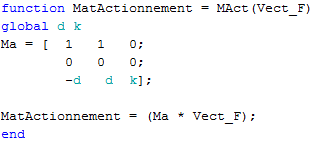
\includegraphics[scale=0.8]{images/actionnement.png}
\caption{Fonction de notre matrice d'actionnement.}
\end{figure}

On remarque que l’on n’a pas de contrôle sur la force de dérive au vu de la disposition des actionneurs sur notre aéroglisseur. 
L'équation que l’on a utilisée pour faire cette matrice est la suivante :

************************* EQUATION **************************

\subsubsection{Modèle dynamique inverse}
\begin{figure}[H]
\bigcenter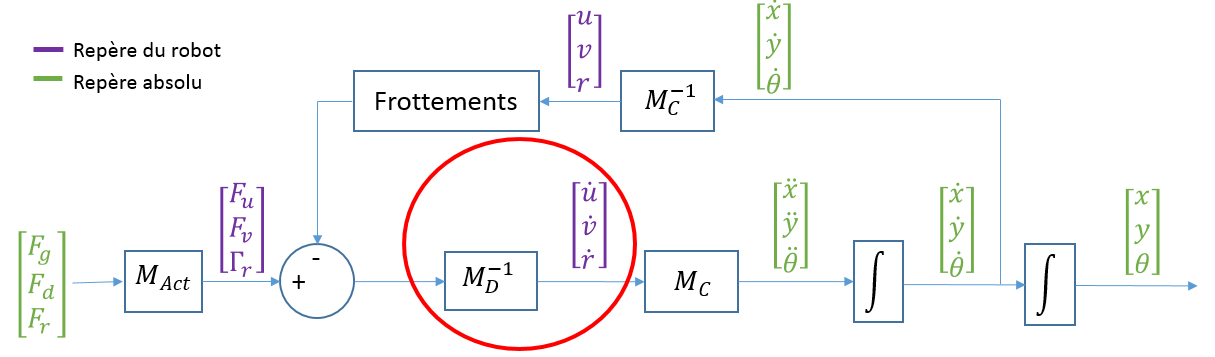
\includegraphics[scale=0.5]{images/modeledynamiqueinverse.png}
\caption{Matrice dynamique inverse.}
\end{figure}

Pour obtenir les accélérations dans le repère du robot, on utilise le modèle dynamique inverse qui est implémenté comme ceci :

\begin{figure}[H]
\bigcenter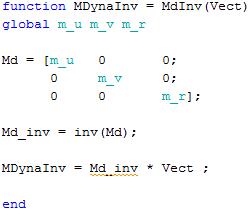
\includegraphics[scale=0.8]{images/dynamique_inverse.png}
\caption{Fonction de notre modèle dynamique inverse.}
\end{figure}

\subsubsection{Modèle cinématique}
\begin{figure}[H]
\bigcenter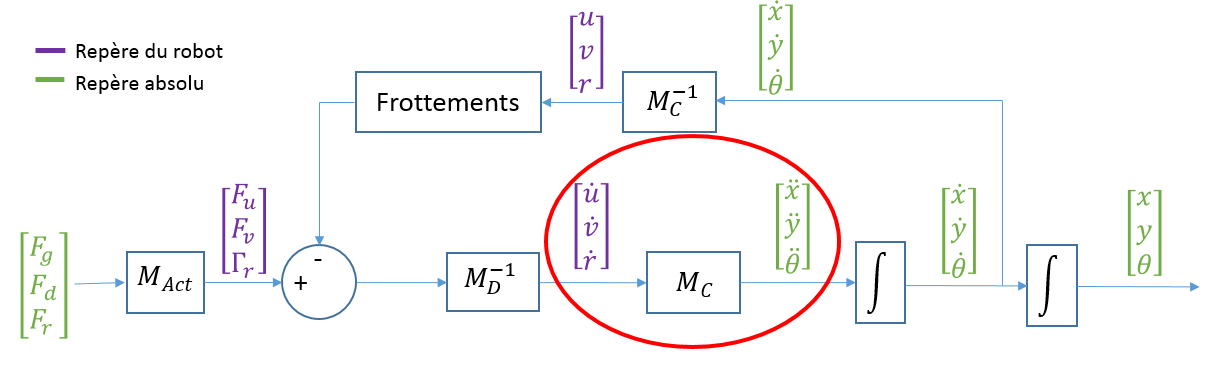
\includegraphics[scale=0.5]{images/modelecinematique.png}
\caption{Matrice dynamique inverse.}
\end{figure}

On repasse aux accélérations dans le repère absolu grâce au modèle cinématique. 

\begin{figure}[H]
\bigcenter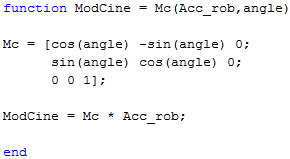
\includegraphics[scale=0.8]{images/cinematique.png}
\caption{Fonction de notre modèle cinématique.}
\end{figure}

Cette fonction prend l’accélération dans le repère du robot et l’angle $\theta$ pour avoir la matrice de rotation actualisée.

\subsubsection{Fonction d'intégration}
\begin{figure}[H]
\bigcenter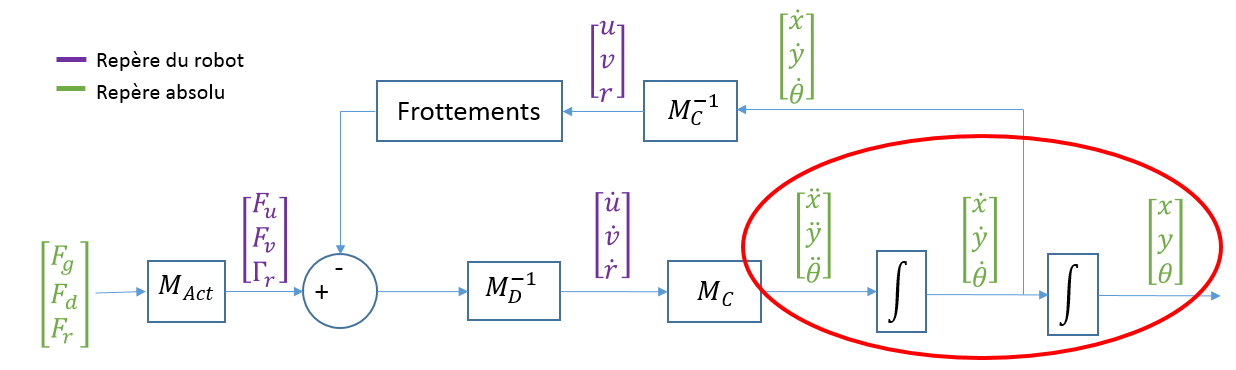
\includegraphics[scale=0.5]{images/integration.png}
\caption{Double intégration.}
\end{figure}

Dans cette partie, il y a une double intégration. On est donc en présence d’un système d’équations différentielles du deuxième ordre. En utilisant ode45 on peut la résoudre en récupérant les vitesses et les positions dans le repère absolu. Voici comment nous avons scindé nos équations dans la fonction appelée par ode45 :

\begin{figure}[H]
\bigcenter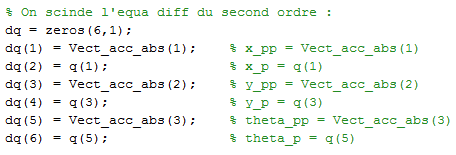
\includegraphics[scale=0.8]{images/double_integration.png}
\caption{Code où l'on scinde l'équation différentielle du second ordre.}
\end{figure}

Ceci n’est pas toute la fonction d’intégration, la fonction entière sera détaillée plus loin.

\subsubsection{Modèle cinématique inverse}
\begin{figure}[H]
\bigcenter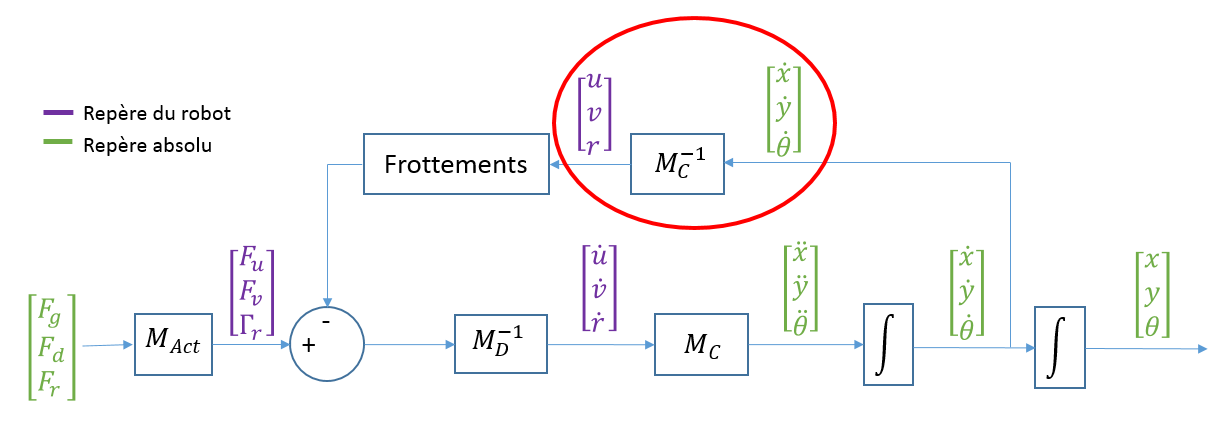
\includegraphics[scale=0.5]{images/modelecinematiqueinverse.png}
\caption{Matrice cinématique inverse.}
\end{figure}

Nous avons choisi de passer par le modèle cinématique inverse pour revenir à nos vitesses dans le plan du robot. Celles-ci sont utilisées pour calculer les frottements subis par notre robot. Voici le code correspondant :

\begin{figure}[H]
\bigcenter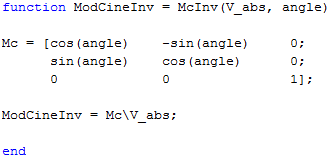
\includegraphics[scale=0.8]{images/cinematique_inverse.png}
\caption{Fonction de notre modèle cinématique inverse.}
\end{figure}

\subsubsection{Boucle globale}
\begin{figure}[H]
\bigcenter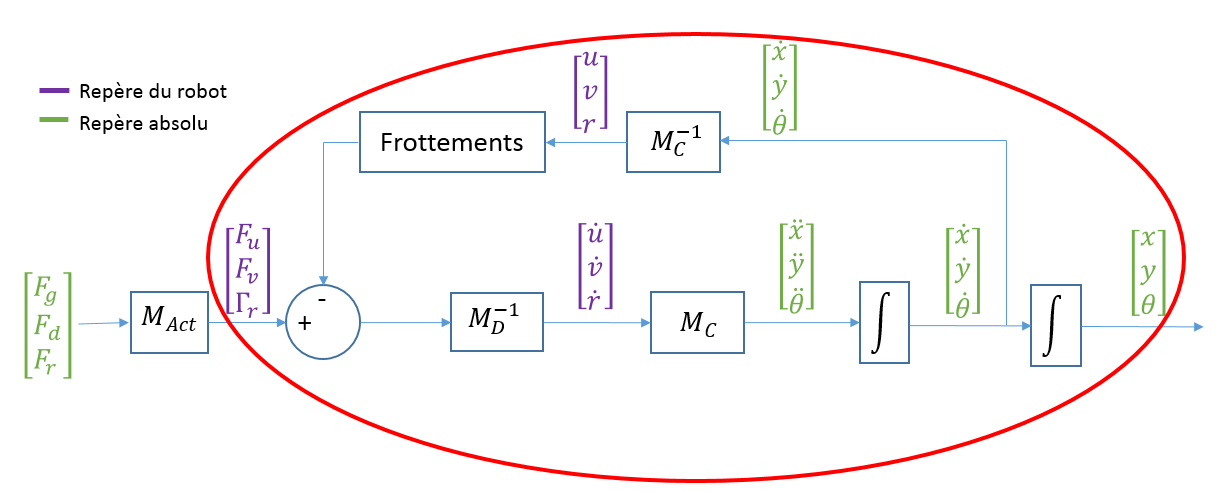
\includegraphics[scale=0.5]{images/boucle_global.png}
\caption{Boucle globale.}
\end{figure}

Notre programme est constitué d’une boucle for qui représente la mise à jour de l’état de notre robot. Elle se compose des étapes classiques d’un simulateur :
\begin{itemize}
\item État de départ (x, y, theta, dx, dy, dtheta)
\item Dessin
\item Calcul de la commande
\item ODE (résolution du système d’équations différentielles du second ordre)
\item Extraction de l’état suivant (qui sera l’état de départ de la prochaine itération de la boucle)
\end{itemize}

\begin{figure}[H]
\bigcenter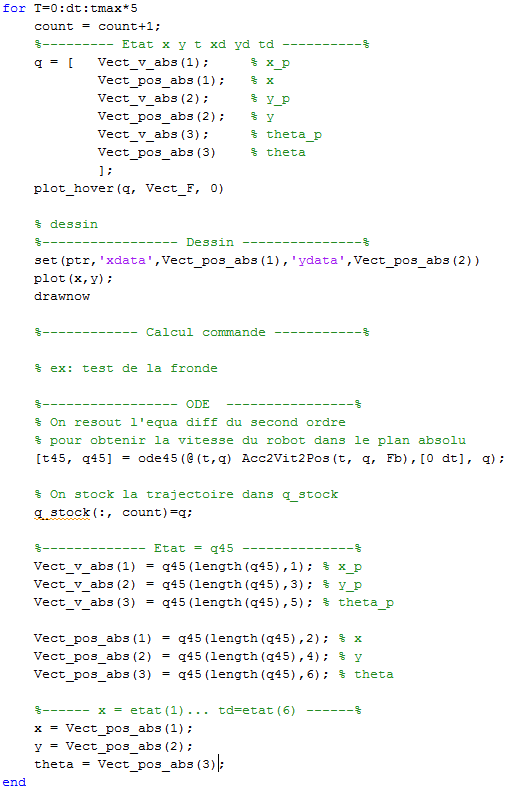
\includegraphics[scale=0.8]{images/boucle_for.png}
\caption{Code de notre boucle globale.}
\end{figure}

Voici la fonction appelée par ode45 :
\begin{figure}[H]
\bigcenter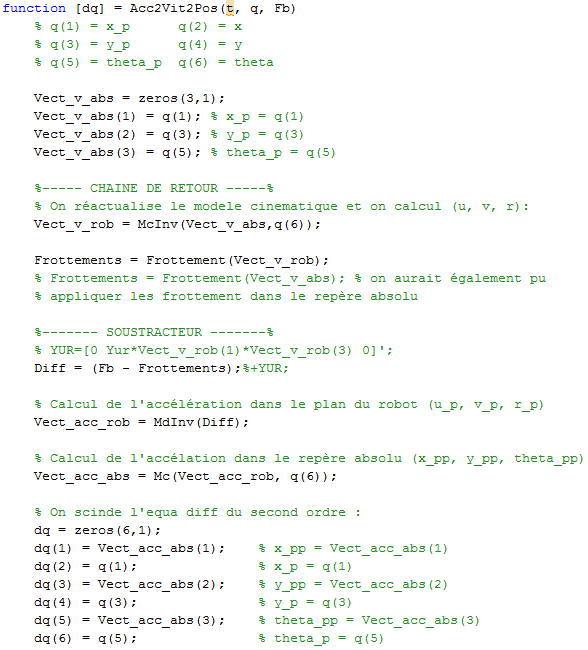
\includegraphics[scale=0.8]{images/Schema_global.png}
\caption{Code de notre boucle globale.}
\end{figure}

On voit qu’à chaque appel de cette fonction par ode on met à jour les variables d’états nécessaires à l’intégration (frottements, orientation, etc.).

\subsubsection{Fonction d'affichage de l'hovercraft}
Nous avons créé une fonction pour afficher l'hovercraft :
\begin{figure}[H]
\bigcenter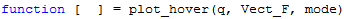
\includegraphics[scale=0.8]{images/plothoverfunction.png}
\end{figure}

Elle prend le vecteur d’état, le vecteur des forces (forces de chaque moteur) ainsi que le mode. Le mode est égal à 1 si c’est le premier appel de la fonction plot\_hover. Cela permet de créer et d’initialiser les objets graphiques. Lorsque le mode est différent de 1, ces objets sont simplement actualisés avec les bonnes valeurs. 

Voici le résultat d’affichage :

\begin{figure}[H]
\bigcenter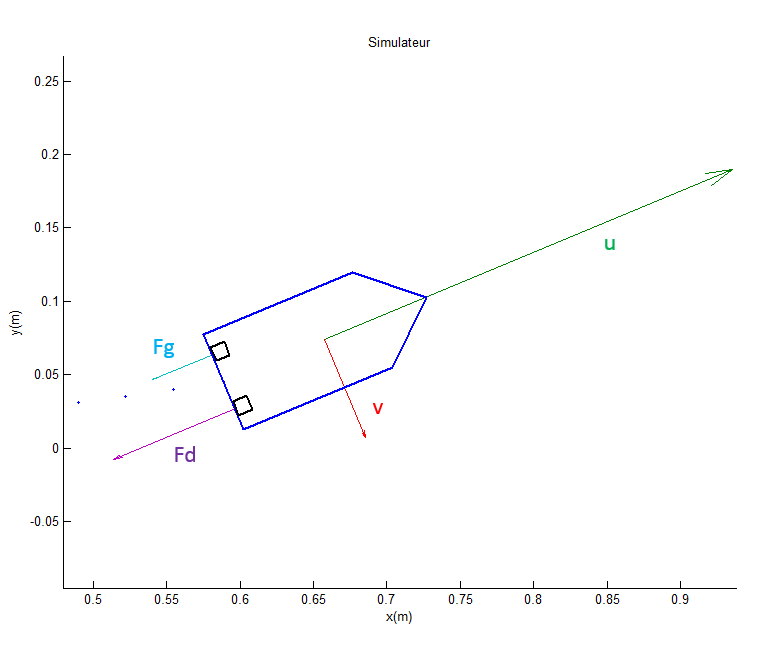
\includegraphics[scale=0.5]{images/plothover.png}
\caption{Affichage de l'hovercraft.}
\end{figure}

$F_g$ et $F_d$ sont les forces de chaque moteurs, $u$ est la force d’avance et $v$ et la force de dérive.

\subsubsection{Résultats}
Voici le résultat obtenu pour une force du moteur gauche égale à la moitié de celle du moteur droit :

\begin{figure}[H]
\bigcenter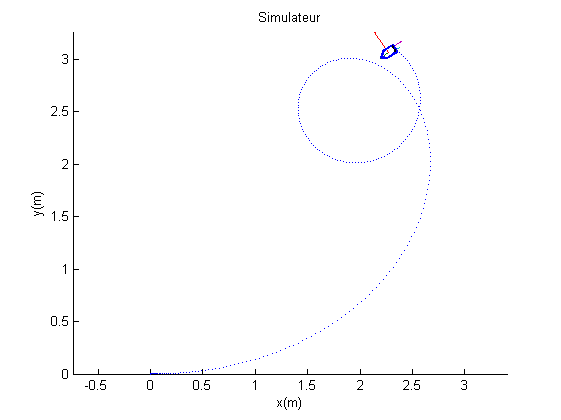
\includegraphics[scale=0.8]{images/simulateur_sortie.png}
\caption{Résulat pour $F_g = 0.5*F_d$.}
\end{figure}

\subsection{Validation (test de la fronde)}

Pour valider notre simulateur, nous avons réalisé le test de la fronde. Pour vérifier que notre système est valide, il faut vérifier que lorsque l’on coupe les moteurs au cours d’un mouvement circulaire, le système doit suivre une trajectoire rectiligne. Voici comment nous l’avons implémenté (dans l'étape du calcul de la commande de notre boucle principale):

\begin{figure}[H]
\bigcenter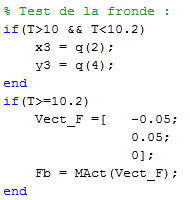
\includegraphics[scale=0.8]{images/fronde_code.png}
\caption{Code du test de la fronde.}
\end{figure}

Et voici le résultat obtenu :
\begin{figure}[H]
\bigcenter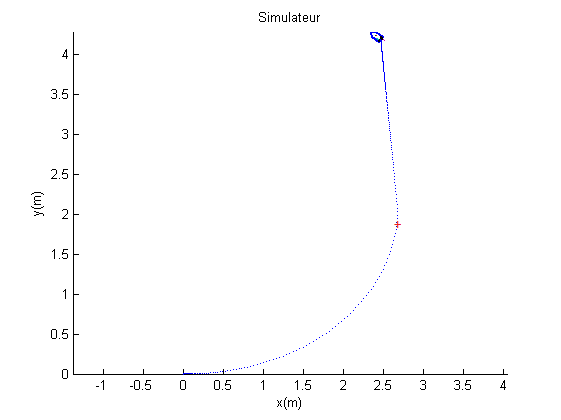
\includegraphics[scale=0.8]{images/fronde.png}
\caption{Résultat du test de la fronde.}
\end{figure}

Le résultat du test valide le simulateur.
%-------------------------------------------------------------------------------------------------------------

\section{Mécanique}


%-------------------------------------------------------------------------------------------------------------

\section{Programmation}

%-------------------------------------------------------------------------------------------------------------

\section{Conclusion}


\end{document}
